\section{Experiments}

\subsection{Experimental setup}
We evaluate our model on both simulated and real-world robotic manipulation tasks. 
To evaluate \ours in simulation, we collected a new dataset for MetaWorld~\citep{yu2020metaworld} comprising of 50 demonstrations for each of the 50 tasks.
For real-world evaluation, we collected three datasets using the SO-100 robot arm~\citep{Knight_Standard_Open_SO-100} and 1 with SO-101 arm~\citep{Knight_Standard_Open_SO-100}, each corresponding to a different manipulation task. Each dataset contains demonstrations relative to one task, with 10 trajectories for each of 5 distinct starting positions, resulting in a total of 50 demonstrations per dataset. The datasets record trajectories relative to
Unless specified otherwise, \ours is always trained in a multi-task setting.

\paragraph{Evaluation metrics.} We report success rate (SR) as the primary metric across all benchmarks. For simulation-based evaluations, SR is binary--set to 1 if the task is successfully completed, and 0 otherwise. For real-world evaluations, we adopt a more fine-grained scoring approach by decomposing each task into subtasks. For example, in the Pick-and-Place task, we assign a score of 0.5 for successfully picking the cube and an additional 0.5 for correctly placing it into the target container.

\paragraph{Simulated environments.}
We evaluate \ours in two established multi-task simulation benchmarks: LIBERO~\citep{liu2023libero} and Meta-World~\citep{yu2020metaworld}. LIBERO assesses diverse visuomotor skills across four categories--\textit{Spatial}, \textit{Object}, \textit{Goal}, and \textit{Long}--with 10 tasks per category (40 total). We use a dataset~\citep{kimopenvla,pertsch2025fast}\footnote{LIBERO dataset: \href{https://huggingface.co/datasets/physical-intelligence/libero}{physical-intelligence/libero}} containing 1,693 episodes covering all tasks, and evaluate with 10 trials per task, reporting average success rates based on binary completion criteria. 
Meta-World evaluates generalization across 50 tasks of varying difficulty: \textit{easy}, \textit{medium}, \textit{hard}, and \textit{very hard}~\citep{seo2023masked}. We use a dataset\footnote{Meta-World dataset: \href{https://huggingface.co/datasets/lerobot/metaworld_mt50}{lerobot/metaworld\_mt50}} of 2,500 episodes (50 per task), and mirror the evaluation protocol used for LIBERO: 10 trials per task, with trials scored as 1 only if the task is fully completed.

\paragraph{Real-world tasks.} We evaluated \ours on 4 datasets in a real-world setting, which we open-source on Hugging Face (\Cref{fig:tasks}). In particular, we benchmark real-world pick and placing capabilities\footnote{Pick-Place dataset: \href{https://huggingface.co/datasets/lerobot/svla_so100_pickplace}{lerobot/svla\_so100\_pickplace}}, stacking capabilities\footnote{Stacking dataset: \href{https://huggingface.co/datasets/lerobot/svla_so100_stacking}{lerobot/svla\_so100\_stacking}.}, and sorting capabilities\footnote{Sorting dataset: \href{https://huggingface.co/datasets/lerobot/svla_so100_sorting}{lerobot/svla\_so100\_sorting}.} for the SO100 robot, alongside real-world pick and placing capabilities for the SO101 platform \footnote{(SO101) Pick-Place dataset: \href{https://huggingface.co/datasets/lerobot/svla_so101_pickplace}{lerobot/svla\_so101\_pickplace}}. Critically, \ours is not pretrained on any datasets recorded for the SO101.

For the pick and place task, \ours is instructed to \texttt{pick up the cube and place it in the box}. The box is small in size and in a fixed position positions while the cube starting position is varied within 5 different starting conditions. % TODO(fracapuano): for the academic submission provide a figure of the different starting positions should be provided
We assess completion of the task with a fine-grained score resulting in a score of 0.5 for successfully grasping the cube, and 0.5 for successfully placing it into the box.
 
For the stacking task, \ours is required to put a cube on top of another. We instruct the robot to \texttt{pick up the red cube and put it on top of the blue cube}. The initial positions of both cubes vary across episodes.
% TODO(fracapuano): for the academic submission provide a figure of the different starting positions should be provided
We assess completion of the task with a fine-grained score resulting in a score of 0.5 for successfully grasping the top cube, and 0.5 for successfully placing it on top of the bottom cube.

For the sorting tasks, which has longer horizon, \ours must sort the cubes depending on the color, following the instruction to \texttt{put the red cube in the right box and the blue cube in the left box}. The cubes are placed in  5 different positions as in Task~1. To introduce variation, the colors of the cubes are flipped, with 5 episodes per color configuration, resulting in 10 demonstrations per position. The boxes locations remain fixed across all demonstrations. 
We assess completion of the task with a fine-grained score resulting in a score of 0.25 for successfully grasping either of the cubes, and 0.25 for successfully completing one cube-box matching, resulting in a score of 0.25 \( \times \) 4 upon task completion.
Figure~\ref{fig:tasks}(A) presents initial and final frames for successful episodes for all tasks, alongside the Hugging Face handle of the corresponding dataset\footnote{Datasets can be easily explored via \href{https://huggingface.co/spaces/lerobot/visualize_dataset}{\texttt{visualize\_dataset}}}.

To assess \ours's generalization, we also evaluate our model on a different robot embodiment and task\footnote{Pick-Place-Lego dataset: \href{https://huggingface.co/datasets/lerobot/svla_so101_pickplace}{lerobot/svla\_so101\_pickplace}.}, similar to pick-place but rather using a small block instead of a cube. 
In this task, the robot is instructed to \texttt{put the pink lego brick into the transparent box}. This task requires more precision, especially in grasping the small lego object, together with advanced vision capabilities considering the box's transparency.

\begin{figure}
    \centering
    \begin{minipage}[t]{0.99\textwidth}
        \centering
        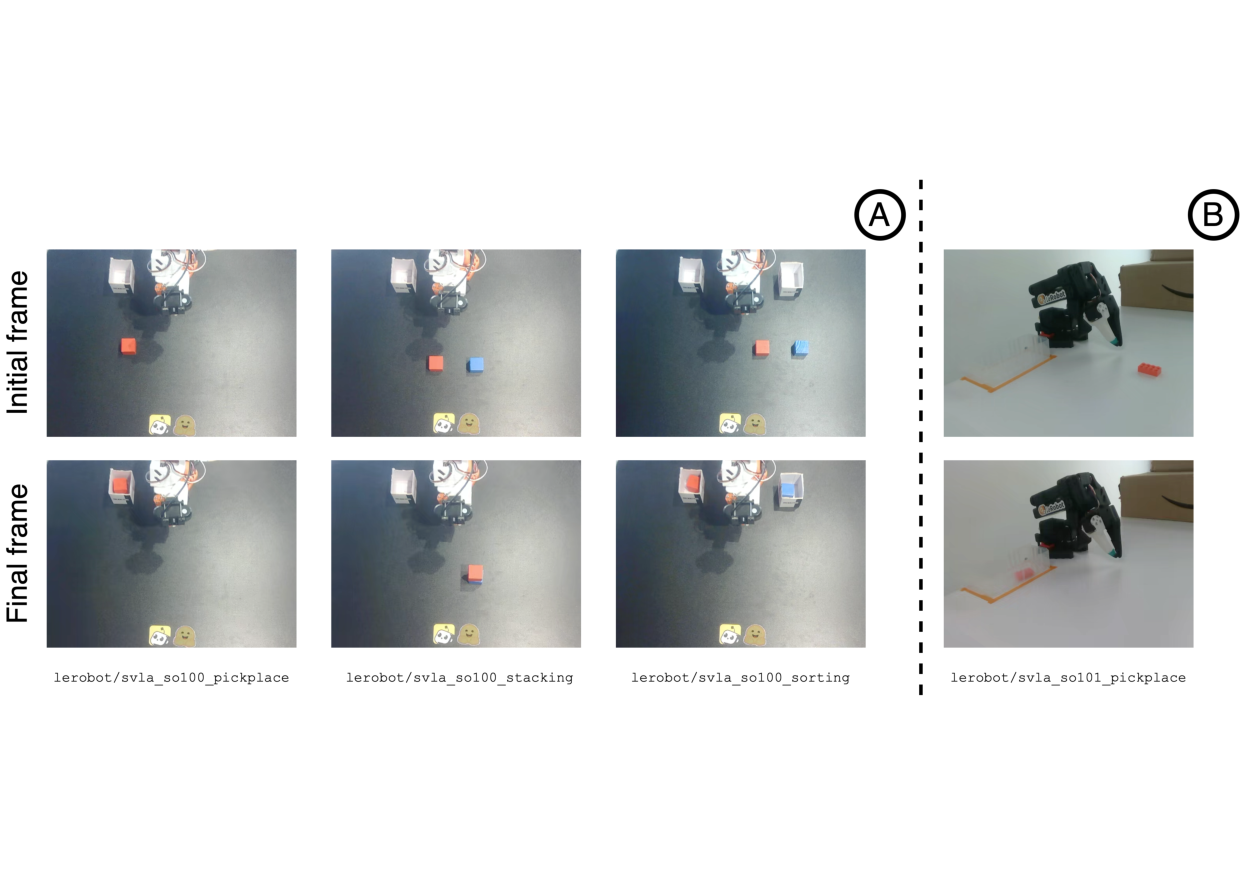
\includegraphics[width=\textwidth]{figures/tasks.pdf}
        \caption{Illustrations of the four real-world tasks we benchmark \ours against, presenting starting and terminal frame for each of the dataset considered, for both SO100 embodiments (A) and SO101 (B). For SO100, we use top and wrist cameras, where for SO101 we use top and side cameras (as seen in the images).}
        \label{fig:tasks}
    \end{minipage}
    \vspace{-0.6cm}
\end{figure}

% \paragraph{LIBERO~\citep{liu2023libero}.}
% LIBERO is a multi-task simulated benchmark designed to test various aspects of VLA capabilities. We evaluate our model across four categories: \textit{Spatial}, \textit{Object}, \textit{Goal}, and \textit{Long}.
% Each category assesses specific skills in the VLA's behavior: spatial relationships are probed by changing object positions, object recognition is assessed by altering object types, goal understanding is tested by modifying the task goal, and long-horizon capabilities are measured measuring long-term capabilities. 
% Each of these categories contains 10 tasks, totaling 40 distinct tasks. Our model is trained on a dataset\footnote{LIBERO dataset: \href{https://huggingface.co/datasets/physical-intelligence/libero}{physical-intelligence/libero}.}~\citep{kimopenvla,pertsch2025fast} covering all these tasks and amounting at 1,693 episodes. 
% For evaluation, we conduct 10 trials per task and report the average success rate. Success rates is computed averaging binary success indicators over each trial, with a score of 1 being awarded exclusively when the robot completes the task correctly (0 otherwise).

% \paragraph{Meta-World \citep{yu2020metaworld}.}
% Meta-World is another multi-task simulation benchmark focused on testing model generalization across 50 different tasks, categorized into varying difficulty levels: \textit{easy}, \textit{medium}, \textit{hard}, and \textit{very hard}~\citep{seo2023masked}. 
% We collect a training dataset \footnote{Meta-World dataset: \href{https://huggingface.co/datasets/lerobot/metaworld_mt50}{lerobot/metaworld\_mt50}.} of 2,500 episodes, with 50 episodes per task. For evaluation, we perform 10 trials per task and report the average success rate. Similar to LIBERO, the tasks are sparse, with a success score of 1 achieved only when the task is fully completed.


\subsection{Robots}
Across simulation and real-world enviroments, we use a variety of robotic platforms.
\begin{itemize}
    \item \textbf{SO100 and SO101 \citep{cadene2024lerobot}}. The Standard Open SO-100 is a low-cost, 3D-printable robotic arm designed for improving accessibility to robotics and robot learning research. Both the SO-100 and its updated version, the SO-101, are open-source platforms for basic manipulation tasks. Each arm has six degrees of freedom and uses low-cost servo motors that are controlled with position commands. The SO101 has better arm design for faster assembly and different motors, making its movements smoother and better for tasks requiring more precisions.
    \item \textbf{Panda \citep{haddadin2022franka}.} The Franka Emika Panda is a single 7-DOF torque-controlled robotic arm designed for safe and precise manipulation. Its high-resolution joint sensing and compliant control make it well-suited for learning-based manipulation tasks in both simulation and real-world settings. This robot is used in the LIBERO simulator.
    \item \textbf{Swayer \citep{yu2020metaworld}.} Is a single 4-DOF controlled robotic arm designed for manipulation tasks. Is is used in the Meta-World simulator and the policy control the position and state of the gripper.    
\end{itemize}

\subsection{Implementation details.}

We conduct our experiments using LeRobot~\citep{cadene2024lerobot}, a PyTorch-based framework for real-world robotics. 
During pretraining, we train for 200,000 steps with a global batch size of 256 on all our community datasets. 
After a 100-step warmup, we use a cosine learning rate schedule starting at 1e-4 and decaying to a minimum of 2.5e-6. We use the AdamW optimizer with $\beta_1=0.9, \beta_2=0.95$.
Training is performed after resizing the images to 512×512, for consistency with the VLM input size. 
We use SmolVLM-2~\citep{marafioti2025smolvlm} as our VLM backbone. 
The action expert is trained with flow matching to output chunks of \( n = 50 \) actions. For real-world evaluation, we perform synchronous inference: the model samples new observations only after executing the full chunk of actions. In simulation, we perform inference by sampling new observations and predicting a new action after each executed action. During inference, the flow matching is fixed to 10 steps. 
We train only the action expert module, keeping the VLM frozen. 
Our main model, contains 450 million parameters, with approximately 100 million dedicated to the action expert. 
We use only the first 16 layers of the large language model (LLM) within the VLM. For fine-tuning on simulation benchmarks, we train for 100,000 steps with a batch size of 64, while for real-world tasks, we fine-tune for 200,000 steps. 
However, we observe in practice that the model can be trained for a much smaller number of steps without sacrificing significant performance levels.

Beyond maintaining a compact model and a reduced number of tokens, we employ several optimizations to enhance training efficiency. 
Specifically, we leverage \texttt{bfloat16} precision and \texttt{torch.compile()} \citep{paszke2019pytorch} that JIT-compiles PyTorch code into optimized kernels. 
To ensure compatibility with these optimizations, we maintain a fixed sequence length and batch size, discarding any excess frames in an episode that do not fit a complete batch. 
For multi-GPU and multi-node training, we utilize Hugging Face's \texttt{accelerate} \citep{accelerate} library with mixed precision, providing a scalable and memory-efficient training setup. 
Pretraining was conducted using 4 GPUs to accomodate for large batch size, but the model can easily be trained on a single GPU due to its small size. Overall, the project consumed approximately 30k GPU hours.

\subsection{Baselines}
We compare our model against two popular and strong baselines, both available in the LeRobot library \citep{cadene2024lerobot}.

\paragraph{\( \bf{\pi}_0 \) \citep{black2024pi_0}.}
\( \pi_0 \) is a VLA which leverages a VLM combined with Flow Matching for action chunk prediction. 
It has a total model size of 3.3 billion parameters and is pre-trained on 10,000 hours of cross-embodiment robotics data. 
The model architecture is based on Paligemma \citep{beyer2024paligemma} and accepts three RGB images, sensorimotor states, and a language instruction as inputs.

\paragraph{ACT \citep{zhao2023learningact}.}
ACT is a Conditional Variational Autoencoder (CVAE) \citep{NIPS2015_8d55a249cvae} policy model with an encoder-decoder transformer architecture containing approximately 80 million parameters. ACT uses a ResNet vision encoder pre-trained on ImageNet, while the CVAE is trained from scratch. The model generates action chunks and is optimized using a regression objective, directly predicting continuous actions. The model accepts a sequence of RGB images, and sensorimotor states.

% \paragraph{Diffusion policy \citep{chi2024diffusionpolicy}.} (TODO: fracapuano) add diffusion policy to the mix for the submission

\subsection{Main results}
In this section, we present the main results of \ours in both real-world and simulated environments. For real-world evaluation, \ours is pretrained on community-collected datasets. \( \pi_0 \) is finetuned on the respective target datasets, while ACT is trained from scratch on each dataset.

% \begin{figure}[h!]
%     \centering
%     \captionsetup{type=figure}

%     \definecolor{grayrow}{gray}{0.92}
    
%     % LIBERO Benchmark Table
%     \begin{minipage}[t]{0.48\linewidth}
%         \centering
%         \setlength{\tabcolsep}{6pt}
%         \renewcommand{\arraystretch}{1.2}
%         \resizebox{\linewidth}{!}{
%         \begin{tabular}{lccccccc}
%             \toprule
%             \textbf{Policy} & \textbf{Model Size} & \textbf{VLA} & \multicolumn{5}{c}{\textbf{Success Rate (\%) — LIBERO}} \\
%             \cmidrule(lr){4-8}
%             & & Pretrain & \textbf{E} & \textbf{M} & \textbf{H} & \textbf{VH} & \textbf{Avg} \\
%             \midrule
%             % \rowcolor{grayrow}
%             % \multicolumn{8}{l}{\textbf{Prior Work}} \\
%             Diffusion Policy & -- & No & 78.3 & 92.5 & 68.3 & 50.5 & 72.4 \\
%             Octo & 0.09B & Yes & 78.9 & 85.7 & 84.6 & 51.1 & 75.1 \\
%             OpenVLA & 7B & Yes & 84.7 & 88.4 & 79.2 & 53.7 & 76.5 \\
%             $\pi_0$ (Paligemma-3B) & 3.3B & No & 87 & 63 & 89 & 48 & 71.8 \\
%             $\pi_0$ & 3.3B & Yes & 90 & 86 & 95 & 73 & 86.0 \\
%             \midrule
%             % \rowcolor{grayrow}
%             % \multicolumn{8}{l}{\textbf{Ours}} \\
%             \ours & 0.45B & No & 90 & 96 & 92 & 71 & \textbf{87.3} \\
%             \bottomrule
%         \end{tabular}
%         }
%         \captionof{table}{\textbf{LIBERO benchmark.} Success rates of different policies on LIBERO. Scores are from \cite{kimopenvla} except for ours.}
%         \label{tab:libero_results}
%     \end{minipage}
%     \hfill
%     % Meta-World Benchmark Table
%     \begin{minipage}[t]{0.48\linewidth}
%         \centering
%         \setlength{\tabcolsep}{6pt}
%         \renewcommand{\arraystretch}{1.2}
%         \resizebox{\linewidth}{!}{
%         \begin{tabular}{lcccccc}
%             \toprule
%             \textbf{Policy} & \textbf{VLA} & \multicolumn{5}{c}{\textbf{Success Rate (\%) — Meta-World}} \\
%             \cmidrule(lr){3-7}
%             & Pretrain & \textbf{S} & \textbf{O} & \textbf{G} & \textbf{10} & \textbf{Avg} \\
%             \midrule
%             % \rowcolor{grayrow}
%             % \multicolumn{7}{l}{\textbf{Prior Work}} \\
%             Diffusion Policy & No & 23.1 & 10.7 & 1.9 & 6.1 & 10.5 \\
%             TinyVLA & No & 77.6 & 21.5 & 11.4 & 15.8 & 31.6 \\
%             $\pi_0^*$ (3.5B-Paligemma) & No & 80.4 & 40.9 & 36.7 & 44.0 & 50.5 \\
%             $\pi_0^*$ (3.5B) & Yes & 71.8 & 48.2 & 41.7 & 30.0 & 47.9 \\
%             \midrule
%             % \rowcolor{grayrow}
%             % \multicolumn{7}{l}{\textbf{Ours}} \\
%             \ours (0.45B) & No & 82.5 & 41.8 & 45.0 & 60.0 & \textbf{57.3} \\
%             \bottomrule
%         \end{tabular}
%         }
%         \captionof{table}{\textbf{Meta-World benchmark.} Comparison on Meta-World. Diffusion policy numbers are from \cite{wen2024tinyvla}.}
%         \label{tab:metaworld_results}
%     \end{minipage}
% \end{figure}

\begin{table}[h!]
    \centering
    \setlength{\tabcolsep}{6pt}
    \renewcommand{\arraystretch}{1.2}
    \definecolor{grayrow}{gray}{0.92}
    \resizebox{0.85\linewidth}{!}{
    \begin{tabular}{llc|ccccc}
        \toprule
        \textbf{Benchmark} & \textbf{Policy (\# Params)} & \textbf{VLA Pt.} & \multicolumn{5}{c}{\textbf{Success Rate (\%) — Simulation}} 
             \\
        \midrule
        \rowcolor{grayrow}
        \multicolumn{3}{l}{\textbf{LIBERO}} & \textbf{Spatial} & \textbf{Object} & \textbf{Goal} & \textbf{Long} & \textbf{Avg.}\\
        & Diffusion Policy \citep{chi2023diffusion}  & No & 78.3 & 92.5 & 68.3 & 50.5 & 72.4 \\
        & Octo (0.09B) \citep{team2024octo} & Yes & 78.9 & 85.7 & 84.6 & 51.1 & 75.1 \\
        & OpenVLA (7B) \citep{kimopenvla} & Yes & 84.7 & 88.4 & 79.2 & 53.7 & 76.5 \\
        & $\pi_0$ (Paligemma-3B) & No & 87 & 63 & 89 & 48 & 71.8 \\
        & $\pi_0$ (3.3B) & Yes & 90 & 86 & 95 & 73 & 86.0 \\
        \midrule
        & \ours (0.24B) & No & 87 & 93 & 88 & 63 & 82.75 \\
        & \ours (0.45B) & No & 90 & 96 & 92 & 71 & 87.3 \\
        & \ours (2.25B) & No & 93	& 94 & 91 & 77 & \textbf{88.75} \\
        \midrule
        \rowcolor{grayrow}
        \multicolumn{3}{l}{\textbf{Meta-World}} & \textbf{Easy} & \textbf{Medium} & \textbf{Hard} & \textbf{Very Hard} & \textbf{Avg.} \\
        & Diffusion Policy \citep{chi2023diffusion} & No & 23.1 & 10.7 & 1.9 & 6.1 & 10.5 \\
        & TinyVLA \citep{TinyLLaVA} & No & 77.6 & 21.5 & 11.4 & 15.8 & 31.6 \\
        & $\pi_0$ (3.5B-Paligemma) & No & 80.4 & 40.9 & 36.7 & 44.0 & 50.5 \\
        & $\pi_0$ (3.5B) & Yes & 71.8 & 48.2 & 41.7 & 30.0 & 47.9 \\
        \midrule
        & \ours (0.24B) & No & 86.43 & 46.36 & 35 & 60 & 56.95 \\
        & \ours (0.45B) & No & 82.5 & 41.8 & 45.0 & 60.0 & 57.3 \\
        & \ours (2.25B) & No & 87.14 & 51.82 & 70 & 64 & \textbf{68.24} \\
        \bottomrule
    \end{tabular}
    }
    \caption{\textbf{Simulation benchmarks (LIBERO and Meta-World).} Success rates (\%) for various policies. LIBERO tasks correspond to different  settings (e.g., spatial, object, goal, long-horizon); Meta-World tasks reflect different difficulty levels. VLA Pt refers pretraining on robotics data. SmolVLA is only initialized from the VLM. Baselines scores from \cite{kimopenvla,wen2024tinyvla}.}
    \label{tab:libero_metaworld_combined}
\end{table}


\paragraph{Simulation Evaluation.}
In \Cref{tab:libero_metaworld_combined}, we further evaluate \ours on two major simulation benchmarks--LIBERO and Meta-World--using a multi-task training setup. \ours{} outperforms other VLA-based approaches such as Octo \citep{team2024octo} and OpenVLA \citep{kimopenvla}, as well as the diffusion policy baseline across both LIBERO and Meta-World. We also compare against two variants of $\pi_0$: one initialized from a vision-language model (Paligemma-3B), and another further pretrained on robotics datasets (intitialized from the weights released by the authors). Despite not being pretrained on robotics data, \ours{} consistently outperforms the VLM-initialized $\pi_0$ and performs competitively with the robotics-pretrained version. Note that, compared to $\pi_0$, \ours is around 40\% faster to train and consumes 6$\times$ less memory.

\begin{table}[h!]
    \centering
    \begin{minipage}[t]{0.52\linewidth}
        \centering
        \setlength{\tabcolsep}{10pt}
        \renewcommand{\arraystretch}{1.1}
        \definecolor{lightgray}{gray}{0.92}
        \resizebox{\linewidth}{!}{
        \begin{tabular}{lcccc}
            \toprule
            & \multicolumn{4}{c}{\textbf{Success Rate (\%) — Real World}} \\
            \cmidrule(lr){2-5}
            \textbf{Policy} & \textbf{Pick-Place} & \textbf{Stacking} & \textbf{Sorting} & \textbf{Avg.} \\
            \midrule
            \rowcolor{lightgray}
            \multicolumn{5}{l}{\textbf{Single-task Training}} \\
            ACT & 70 & 50 & 25 & 48.3 \\
            \midrule
            \rowcolor{lightgray}
            \multicolumn{5}{l}{\textbf{Multi-task Training}} \\
            $\pi_0$ (3.5B)       & 100 & 40 & 45 & 61.7 \\
            \ours (0.45B)         & 75 & 90 & 70 & 78.3 \\
            \bottomrule
        \end{tabular}
        }
        \caption{\textbf{Real-world benchmarks (SO100).} Success rate (\%) across three tasks using policies trained in multi-task and single-task settings.}
        \label{tab:main_results_real}
    \end{minipage}%
    \hspace{0.05\linewidth}%
    \begin{minipage}[t]{0.38\linewidth}
        \centering
        \setlength{\tabcolsep}{8pt}
        \renewcommand{\arraystretch}{1.2}
        \definecolor{lightgray}{gray}{0.92}
        \resizebox{\linewidth}{!}{
        \begin{tabular}{lcc}
            \toprule
            & \multicolumn{2}{c}{\textbf{Success Rate (\%) — Real World}} \\
            \cmidrule(lr){2-3}
            \textbf{Policy} & \textbf{In Distribution} & \textbf{Out of Distribution} \\
            \midrule
            \rowcolor{lightgray}
            \multicolumn{3}{l}{\textbf{Single-task Training}} \\
            ACT & 70 & 40 \\
            % \midrule
            % \rowcolor{lightgray}
            % \multicolumn{3}{l}{\textbf{Multi-task Training}} \\
            \ours (0.45B)  & 90 & 50 \\
            \bottomrule
        \end{tabular}
        }
        \caption{\textbf{Real-world benchmark (SO101).} Success rate (\%) for the Pick-Place-Lego task using policies trained in single-task setting.}
        \label{tab:main_results_real_so101}
    \end{minipage}
\end{table}


\paragraph{Real-World Evaluation.}
In \Cref{tab:main_results_real}, we evaluate \ours{} on four real-world tasks. For the SO101 benchmark, the model is trained on a combination of three datasets, and success rates are reported per task as well as on average. \ours{} outperforms both ACT \citep{zhao2023learningact}, which is trained individually on each task, and \( \pi_0 \), a significantly larger model in terms of parameter count (\( \sim 7\times\)). 
Similarly, on SO101 (see \Cref{tab:main_results_real_so101}), \ours{} surpasses ACT in both in-distribution and out-of-distribution (OOD) settings. For OOD evaluation, the Lego object is placed in novel positions not previously encountered during training.

\begin{table}[h!]
    \centering
    \begin{minipage}[t]{0.95\linewidth}
        \centering
        \setlength{\tabcolsep}{10pt}
        \renewcommand{\arraystretch}{1.1}
        \definecolor{lightgray}{gray}{0.92}
        \resizebox{0.7\linewidth}{!}{
        \begin{tabular}{lccccc}
            \toprule
            & & \multicolumn{4}{c}{\textbf{Success Rate (\%) — Real World}} \\
            \cmidrule(lr){3-6}
            \textbf{Policy} & \textbf{VLA pt.} &  \textbf{Pick-Place} & \textbf{Stacking} & \textbf{Sorting} & \textbf{Avg.} \\
            \midrule
            \rowcolor{lightgray}
            \multicolumn{6}{l}{\textbf{Single-task Training}} \\
            \ours (0.45B)   & No & 55 & 45 & 20 & 40 \\
            \midrule
            \rowcolor{lightgray}
            \multicolumn{6}{l}{\textbf{Multi-task Training}} \\
            \ours (0.45B)    & No   & 80 & 40 & 35 & 51.7 \\
            \ours (0.45B)    & Yes  & 75 & 90 & 70 & 78.3 \\
            \bottomrule
        \end{tabular}
        }
        \caption{\textbf{Effect of pretraining and multitask learning.} Success rate (\%) across three tasks using \ours trained in multi-task and single-task settings. Results with SO100 robot.}
        \label{tab:main_results_effect_of_pretrain}
    \end{minipage}%
    \hspace{0.05\linewidth}%

\end{table}


\paragraph{Effect of pretraining and multitask learning.} In \Cref{tab:main_results_effect_of_pretrain}, we further evaluate the impact of pretraining \ours on community datasets in terms of the difference in real-world performance, and investigate whether multitask finetuning provides additional benefits for \ours. The results show that, pretraining on community datasets leads to a substantial performance improvement (from 51.7 to 78.3). 
Furthermore, multitask finetuning yields further gains, underscoring the importance of knowledge transfer across tasks.

% Diffusion Policy~\cite{khazatsky2024droid} libero

% Diffusion Policy~\cite{chi2023diffusion} metaworld

% \begin{itemize}
%     \item Figure 1: Performance (AVG SR) vs training time.
%     \item Figure 2: Performance vs inference time.
% \end{itemize}

% \begin{table}[h!]
    \centering
    \setlength{\tabcolsep}{12pt}
    \renewcommand{\arraystretch}{1.3}
    \definecolor{lightgray}{gray}{0.92}
    \resizebox{0.4\linewidth}{!}{
    \begin{tabular}{lcc}
        \toprule
        \textbf{Policy} & \multicolumn{2}{c}{\textbf{Pick-Place-Lego}}  \\
        & ID & OOD \\ \cmidrule{1-2}
        \midrule
        \rowcolor{lightgray}
        \multicolumn{3}{l}{\textbf{Single-task Training}} \\
        \quad ACT~\citep{zhao2023learningact}  & 70 & 40 \\
        \midrule
        \rowcolor{lightgray}
        \multicolumn{3}{l}{\textbf{Multi-task Training}} \\
        \quad \ours-450M         & 90 & 50 \\
        \bottomrule
    \end{tabular}
    }
    \caption{\textbf{Real-world evaluation on SO101 and SO101 OOD.} Success rate (\%) across the Pick-Place-Lego task using policies trained in single-task and multi-task settings. For OOD evaluation, the Lego is shifted by around 1 cm from the training position.}
    \label{tab:combined_results_real_so101}
\end{table}


% \begin{figure}[h!]
%     \centering
%     \captionsetup{type=figure}

%     \begin{minipage}[t]{0.42\linewidth}
%         \centering
%         \setlength{\tabcolsep}{5pt}
%         \renewcommand{\arraystretch}{1.2}
%         \resizebox{0.95\linewidth}{!}{
%         \begin{tabular}{lcccc}
%             \toprule
%             \multirow{2}{*}{\textbf{Inference}} & \multicolumn{4}{c}{\textbf{Success Rate (\%)}} \\\cmidrule(lr){2-5}
%              & \textbf{Pick-Place} & \textbf{Stacking} & \textbf{Sorting} & \textbf{Avg} \\
%             \midrule
%             Sync  & 75 & 70 & 90 & 78.3 \\
%             Async & 80 & 50 & 90 & 73.3 \\
%             \bottomrule
%         \end{tabular}
%         }
%         \captionof{table}{\textbf{Real-world benchmarks.} Both inference modes perform comparably.}
%         \label{tab:real_async_success}
%     \end{minipage}
%     \hfill
%     \begin{minipage}[t]{0.28\linewidth}
%         \centering
%         \setlength{\tabcolsep}{5pt}
%         \renewcommand{\arraystretch}{1.2}
%         \resizebox{0.95\linewidth}{!}{
%         \begin{tabular}{lccc}
%             \toprule
%             \multirow{2}{*}{\textbf{Inference}} & \multicolumn{3}{c}{\textbf{Time (s)}} \\\cmidrule(lr){2-4}
%              & \textbf{Total} & \textbf{Avg} & \textbf{Std} \\
%             \midrule
%             Sync  & 137.5 & 13.75 & 2.42 \\
%             Async & 97.0  & 9.70  & 2.95 \\
%             \bottomrule
%         \end{tabular}
%         }
%         \captionof{table}{\textbf{Pick-Place task completion time.} The robot is faster with asynchronous inference .}
%         \label{tab:real_async_time}
%     \end{minipage}
%     \hfill
%     \begin{minipage}[t]{0.28\linewidth}
%         \centering
%         \setlength{\tabcolsep}{5pt}
%         \renewcommand{\arraystretch}{1.2}
%         \resizebox{0.95\linewidth}{!}{
%         \begin{tabular}{lccc}
%             \toprule
%             \multirow{2}{*}{\textbf{Inference}} & \multicolumn{3}{c}{\textbf{\# of Cubes}} \\\cmidrule(lr){2-4}
%              & \textbf{Total} & \textbf{Avg} & \textbf{Std} \\
%             \midrule
%             Sync  & 19  & 3.8  & 1.3  \\
%             Async & 9   & 1.8  & 0.45 \\
%             \bottomrule
%         \end{tabular}
%         }
%         \captionof{table}{\textbf{Pick-Place in fixed time frame.} Asynchronous inference helps the model to pick and place more cubes in 60 seconds.}
%         \label{tab:real_async_cubes}
%     \end{minipage}
% \end{figure}

\begin{figure}[h!]
    \centering

    \begin{subfigure}[t]{0.42\linewidth}
        \centering
        \setlength{\tabcolsep}{5pt}
        \renewcommand{\arraystretch}{1.2}
        \resizebox{0.95\linewidth}{!}{
        \begin{tabular}{lcccc}
            \toprule
            \multirow{2}{*}{\textbf{Inference}} & \multicolumn{4}{c}{\textbf{Success Rate (\%) — Real World}} \\\cmidrule(lr){2-5}
             & \textbf{Pick-Place} & \textbf{Stacking} & \textbf{Sorting} & \textbf{Avg} \\
            \midrule
            Sync  & 75 & 90 & 70 & 78.3 \\
            Async & 80 & 90 & 50 & 73.3 \\
            \bottomrule
        \end{tabular}
        }
        \subcaption{\textbf{Performance (success rates).}}
        \label{tab:real_async_success}
    \end{subfigure}
    \hfill
    \begin{subfigure}[t]{0.28\linewidth}
        \centering
        \setlength{\tabcolsep}{5pt}
        \renewcommand{\arraystretch}{1.2}
        \resizebox{0.95\linewidth}{!}{
        \begin{tabular}{lccc}
            \toprule
            \multirow{2}{*}{\textbf{Inference}} & \multicolumn{3}{c}{\textbf{Time (s) — Real World}} \\\cmidrule(lr){2-4}
             & \textbf{Total} & \textbf{Avg} & \textbf{Std} \\
            \midrule
            Sync  & 137.5 & 13.75 & 2.42 \\
            Async & 97.0  & 9.70  & 2.95 \\
            \bottomrule
        \end{tabular}
        }
        \subcaption{\textbf{Task completion time.}}
        \label{tab:real_async_time}
    \end{subfigure}
    \hfill
    \begin{subfigure}[t]{0.28\linewidth}
        \centering
        \setlength{\tabcolsep}{5pt}
        \renewcommand{\arraystretch}{1.2}
        \resizebox{0.95\linewidth}{!}{
        \begin{tabular}{lccc}
            \toprule
            \multirow{2}{*}{\textbf{Inference}} & \multicolumn{3}{c}{\textbf{\# of Cubes — Real World} } \\\cmidrule(lr){2-4}
             & \textbf{Total} & \textbf{Avg} & \textbf{Std} \\
            \midrule
            Sync  & 9   & 1.8  & 0.45  \\
            Async & 19  & 3.8  & 1.3  \\
            \bottomrule
        \end{tabular}
        }
        \subcaption{\textbf{Performance in fixed time.}}
        \label{tab:real_async_cubes}
    \end{subfigure}

    \caption{\textbf{Comparison between synchronous (Sync) and asynchronous (Async) inference.} We evaluate \ours on three real-world tasks under both inference modes. Asynchronous inference achieves similar success rates (left) but is significantly faster (middle) and complete more tasks (right) in fixed-time settings. Hyperparameters have been optimized for Pick-Place and reused across tasks.}
    \label{fig:async_inference_summary}
\end{figure}


\subsection{Asynchronous inference}

We evaluated \ours{} under two inference modes: sync and async. 
The sync mode reflects a standard evaluation setting in robotics, whereby the policy predicts a chunk of actions that is executed fully before the next prediction cycle begins. In contrast, the async mode decouples action execution and policy inference, allowing predictions and control to run in parallel.

\paragraph{Results.}
For both inference modes, we report the success rate and policy speed (\Cref{fig:async_inference_summary}). To evaluate speed, we design two experiments using the Pick-Place task. In the first experiment, we measure the time taken to complete the task across 10 trials and 5 different cube positions. In the second, we fix a time limit (e.g., 60 seconds) and count the number of cubes successfully picked and placed into the box, from different positions. Timing begins when the robot starts moving. As shown in \Cref{tab:real_async_success}, both inference modes achieve comparable success rates across three real-world tasks. However, asynchronous inference demonstrates a substantial speed advantage (\Cref{tab:real_async_time}). On average, it completes the task in 9.7 seconds, compared to 13.75 seconds in the synchronous setting (\( \sim 30\% \) faster). Furthermore, under the fixed-time evaluation, the asynchronous mode allows the robot to complete 19 successful pick-and-place cycles, compared to only 9 in the synchronous case (\Cref{tab:real_async_cubes}). Qualitatively, we observe that asynchronous inference enables faster reactions and better adaptability to changes in the environment. The robot exhibits greater robustness to shifts in object positions and external disturbances, and overall is capable to solve the same tasks a significantly larger number of times due to the avoidance of prediction lags (\Cref{fig:async_inference_summary}).

% We start counting the time after the robot move
% for timing we consider always success

% \subsection{SmolVLA on single GPU.}

% No pretraining, direct finetuning on final tasks.

% \subsection{SmolVLA trained on community datasets}

% Pretraining on filtered So100 datasets and then finetuning on the final tasks.


% \subsection{SmolVLA trained on academic and community datasets}

% Large-scale pretraining on academic (+ community) datasets. Then finetuning on final tasks.

\subsection{Ablation Study}
We conduct a comprehensive ablation study to assess key design choices behind the final \ours model. 
All ablations are conducted on the LIBERO benchmark. Unless otherwise noted, models are trained from scratch without any pretraining on robotics data. The VLM backbone is frozen, and only the action expert is trained from scratch.

\begin{figure}[h!]
    \centering
    \captionsetup{type=figure}
    
    \begin{minipage}[t]{0.48\linewidth}
        \centering
        \setlength{\tabcolsep}{6pt}
        \renewcommand{\arraystretch}{1.1}
        \resizebox{0.85\linewidth}{!}{
        \begin{tabular}{cccccc}
            \toprule
            \textbf{Attention} & \multicolumn{5}{c}{\textbf{Success Rate (\%) — LIBERO}} \\ \cmidrule(lr){2-6}
            \textbf{mechanism} & \textbf{S} & \textbf{O} & \textbf{G} & \textbf{10} & \textbf{Avg} \\
            \midrule
            CA             & 87 & 92 & 83 & 54 & 79.0 \\
            SA             & 80 & 94 & 84 & 40 & 74.5 \\
            CA+SA (ours)   & 86 & 99 & 90 & 67 & 85.5 \\
            \bottomrule
        \end{tabular}
        }
        \captionof{table}{\textbf{Cross vs self-attention.} Interleaved cross (CA) and self-attention (SA) yield the best results. 
        % Batch size = 64.
        }
        \label{tab:ablation_model_attention}
    \end{minipage}
    \hfill
    \begin{minipage}[t]{0.48\linewidth}
        \centering
        \setlength{\tabcolsep}{6pt}
        \renewcommand{\arraystretch}{1.1}
        \resizebox{0.8\linewidth}{!}{
        \begin{tabular}{cccccc}
            \toprule
            \textbf{Attention} & \multicolumn{5}{c}{\textbf{Success Rate (\%) — LIBERO}} \\ \cmidrule(lr){2-6}
             \textbf{mask} & \textbf{S} & \textbf{O} & \textbf{G} & \textbf{10} & \textbf{Avg} \\
            \midrule
            Bidir   & 79 & 86 & 82 & 23 & 67.5 \\
            Causal  & 80 & 94 & 84 & 40 & 74.5 \\
            \bottomrule
        \end{tabular}
        }
        \captionof{table}{\textbf{Bidirectional vs causal attention.} Preventing future action leakage improves performance. 
        % Batch size = 64.
        }
        \label{tab:ablation_causal_bidir_attention}
    \end{minipage}
\end{figure}


\paragraph{Cross-attention (CA) vs. self-attention (SA) between VLM and \( \actionexpert \).}
We compare how the VLM features interact with the action expert, comparing causal self-attention (SA), cross-attention (CA), or our proposed interleaved SA+CA setup. 
In the SA setting, action tokens attend to each other using a causal mask, while in the CA setting the VLM features act as keys and values for attention in the \( \actionexpert \). 
As shown in \Cref{tab:ablation_model_attention}, cross-attention outperforms self-attention significantly. Interleaving both yields the best results, highlighting their complementary strengths.

\begin{figure}[h!]
    \centering
    \captionsetup{type=figure}

    \begin{minipage}[t]{0.48\linewidth}
        \centering
        \setlength{\tabcolsep}{6pt}
        \renewcommand{\arraystretch}{1.2}
        \resizebox{0.8\linewidth}{!}{
        \begin{tabular}{cccccc}
            \toprule
            \multirow{2}{*}{\textbf{N}} & \multicolumn{5}{c}{\textbf{Success Rate (\%) — LIBERO}} \\\cmidrule(lr){2-6}
             & \textbf{S} & \textbf{O} & \textbf{G} & \textbf{10} & \textbf{Avg} \\
            \midrule
            8           & 77 & 88 & 86 & 49 & 75.0  \\
            16          & 88 & 91 & 91 & 44 & 78.5  \\
            24          & 86 & 97 & 86 & 49 & 79.5  \\
            32          & 89 & 94 & 85 & 53 & 80.3  \\
            \midrule
            Skip \%2     & 84 & 90 & 83 & 45 & 75.5  \\
            \midrule
            VLM-256M     & 86 & 83 & 75 & 59 & 75.8  \\
            \bottomrule
        \end{tabular}
        }
        \captionof{table}{\textbf{Skipping VLM layers.} Skipping layers from a large VLM (here 500M parameters) yields better results than downsizing the VLM. Skipping every second layer is a competitive baseline.}
        \label{tab:ablation_vlm_layers}
    \end{minipage}
    \hfill
    \begin{minipage}[t]{0.48\linewidth}
        \centering
        \setlength{\tabcolsep}{6pt}
        \renewcommand{\arraystretch}{1.2}
        \resizebox{0.8\linewidth}{!}{
        \begin{tabular}{cccccc}
            \toprule
            \textbf{Expert width} & \multicolumn{5}{c}{\textbf{Success Rate (\%) — LIBERO}} \\\cmidrule(lr){2-6}
             \textbf{(w.r.t. VLM)} & \textbf{S} & \textbf{O} & \textbf{G} & \textbf{10} & \textbf{Avg} \\
            \midrule
            $\times$1.00 & 87 & 96 & 90 & 56 & 82.3 \\
            $\times$0.75 & 82 & 89 & 84 & 55 & 77.5 \\
            $\times$0.50 & 89 & 94 & 85 & 53 & 80.3 \\
            $\times$0.25 & 76 & 97 & 83 & 39 & 73.8 \\
            \bottomrule
        \end{tabular}
        }
        \captionof{table}{\textbf{Expert capacity.} Adjusting the expert's hidden size affects performance. Larger capacities yield better success rates.}
        \label{tab:ablation_expert_capacity}
    \end{minipage}
    
    % \vspace{0.5cm}

    % \begin{minipage}[t]{0.45\linewidth}
    %     \centering
    %     \setlength{\tabcolsep}{6pt}
    %     \renewcommand{\arraystretch}{1.2}
    %     \resizebox{1.0\linewidth}{!}{
    %     \begin{tabular}{lccccc}
    %         \toprule
    %         \textbf{Expert Variant} & \multicolumn{5}{c}{\textbf{Success Rate (\%) — LIBERO}} \\\cmidrule(lr){2-6}
    %          & \textbf{S} & \textbf{O} & \textbf{G} & \textbf{10} & \textbf{Avg} \\
    %         \midrule
    %         Full             & 89 & 94 & 85 & 53 & 80.3  \\
    %         Skip 1 Layer     & 84 & 90 & 83 & 45 & 75.5  \\
    %         VLM-256M         & 86 & 83 & 75 & 59 & 75.8  \\
    %         \bottomrule
    %     \end{tabular}
    %     }
    %     \captionof{table}{\textbf{Shallower action expert.} Using a shallower expert reduces performance compared to the full version, though smaller VLMs with full experts perform similarly.}
    %     \label{tab:ablation_shallow_expert}
    % \end{minipage}
\end{figure}


\paragraph{Causal vs. bidirectional attention on action tokens within \( \actionexpert \).} 
Next, we investigate how action tokens should attend to each other within the action expert, \( \actionexpert \). 
We compare: \emph{(i)} no interaction between action tokens (pure CA), \emph{(ii)} causal self-attention, and \emph{(iii)} bidirectional self-attention. \Cref{tab:ablation_causal_bidir_attention} shows causal self-attention performs best, while bidirectional interaction harms performance.
Surprisingly, the no-interaction (CA-only) setup performs competitively, suggesting that conditioning on VLM features alone can be powerful.

\paragraph{Using early LLM layers in the VLM.}
The VLM backbone consists of a vision encoder followed by an LLM. 
Motivated by improving the efficiency of \ours, we investigate using features from the first \( N < L\) layers only instead of all the \( L \) LLM layers available or the features~\citep{black2024pi_0}.
Before starting to train, we discard the top \( L - N \) layers of the VLM. 
As shown in \Cref{tab:ablation_vlm_layers}, using only the first half of the VLM layers gives a good trade-off between performance and compute. 
Further, we also test a variant sampling every second VLM layer (Skip \% 2, ~\citep{shukor2024skipping})--reducing depth by half while retaining full model capacity. \Cref{tab:ablation_vlm_layers} indicates skipping every second layer performs better than training a smaller VLM, but worse than using the first \( N < L \) layers directly.

% % \vspace{-0.6cm}
% \begin{wraptable}{r}{0.5\linewidth}
%     \centering
%     \setlength{\tabcolsep}{8pt} % Balanced spacing
%     \renewcommand{\arraystretch}{1.2} % Enhanced row height
%     \resizebox{0.8\linewidth}{!}{
%         \begin{tabular}{cccccc}
%         \toprule
%             \textbf{Training objective} & \multicolumn{5}{c}{\textbf{Success Rate (\%) -- LIBERO}} \\\cmidrule(lr){2-6}
%              & \textbf{S} & \textbf{O} & \textbf{G} & \textbf{10} & \textbf{Avg} \\
%             \midrule
%              Flow matching   & 89 & 94 & 85 & 53 & 80.25 \\
%              % \shline
%              Regression   &  92	& 85 & 86 & 38 & 75.25 \\
%         \end{tabular}%
%         }
%         \captionof{table}{\textbf{Training objective.} We compare our training objective based on Flow matching to regression with L1 loss.}
%     \vspace{-0.cm}
%     \label{tab:ablation_regression}
% \end{wraptable}


\paragraph{Action Expert Capacity.}
Motivated by efficiency arguments, we investigate varying the hidden dimension of the action expert to explore the impact of model capacity on performance.
Given the VLM dimension \( d \), \Cref{tab:ablation_expert_capacity} shows reducing the expert's hidden size to \( 0.75 \times d \) achieves a good balance between performance and efficiency.

\begin{figure}[h!]
    \centering
    \captionsetup{type=figure}
    \begin{minipage}[t]{0.48\linewidth}
        \centering
        \setlength{\tabcolsep}{6pt}
        \renewcommand{\arraystretch}{1.2}
        \resizebox{0.9\linewidth}{!}{
            \begin{tabular}{cccccc}
            \toprule
                \textbf{Training} & \multicolumn{5}{c}{\textbf{Success Rate (\%) — LIBERO}} \\\cmidrule(lr){2-6}
                \textbf{objective} & \textbf{S} & \textbf{O} & \textbf{G} & \textbf{10} & \textbf{Avg} \\
                \midrule
                 Flow matching   & 89 & 94 & 85 & 53 & 80.25 \\
                 % \shline
                 Regression   &  92	& 85 & 86 & 38 & 75.25 \\
            \bottomrule
            \end{tabular}%
            }
            \captionof{table}{\textbf{Training objective.} We compare our training objective based on Flow matching to regression with L1 loss.}
        % \vspace{-0.cm}
        \label{tab:ablation_regression}
    \end{minipage}
    \hfill
    \begin{minipage}[t]{0.48\linewidth}
        \centering
        \setlength{\tabcolsep}{6pt}
        \renewcommand{\arraystretch}{1.2}
        \resizebox{0.8\linewidth}{!}{
            \begin{tabular}{ccccccc}
                \toprule
                \textbf{States} & \textbf{Attention} & \multicolumn{5}{c}{\textbf{Success Rate (\%) — LIBERO}} \\\cmidrule(lr){3-7}
                 & & \textbf{S} & \textbf{O} & \textbf{G} & \textbf{10} & \textbf{Avg} \\
                \midrule
                Prefix & CA & 89 & 94 & 85 & 53 & 80.3 \\
                Suffix & CA & 86 & 82 & 78 & 47 & 73.3 \\
                Prefix & SA & 62 & 74 & 57 & 20 & 53.3 \\
                Suffix & SA & 80 & 92 & 80 & 47 & 74.8 \\
                \bottomrule
            \end{tabular}
        }
        \captionof{table}{\textbf{States as prefix vs. suffix.} Feeding states to the VLM (prefix) leads to better performance than feeding them to the expert (suffix).}
        % \vspace{-1cm}
        \label{tab:ablation_states_to_prefix}
    \end{minipage}
\end{figure}


\paragraph{Regression vs. Flow Matching training objectives.}
We compare two learning objectives for training the action expert \( \actionexpert \): flow matching (our default), and a standard regression L1 loss on the predicted versus ground-truth action chunks. 
In keeping with~\citet{black2024pi_0, chi2024diffusionpolicy} \Cref{tab:ablation_regression} shows that flow matching significantly outperforms regression, suggesting flow matching provides better inductive bias for modeling complex, multimodal action distributions.

\paragraph{States to the VLM or Action Expert?}
We compare two variants: \emph{(i)} feeding the sensorimotor states to the VLM (by projecting them into token space), and \emph{(ii)} passing them directly to the action expert. 
\Cref{tab:ablation_states_to_prefix} indicates including state information in the VLM leads to significantly better performance for both the CA and SA variants.

\begin{figure}[h!]
    \centering
    \captionsetup{type=figure}
    
    \begin{minipage}[t]{0.48\linewidth}
        \centering
        \setlength{\tabcolsep}{6pt}
        \renewcommand{\arraystretch}{1.2}
        \resizebox{0.7\linewidth}{!}{
        \begin{tabular}{cccccc}
            \toprule
            \textbf{Chunk} & \multicolumn{5}{c}{\textbf{Success Rate (\%) — LIBERO}} \\\cmidrule(lr){2-6}
            \textbf{Size} & \textbf{S} & \textbf{O} & \textbf{G} & \textbf{10} & \textbf{Avg} \\
            \midrule
             1   & 45 & 77 & 54 & 24 & 50.0  \\
             10  & 90 & 94 & 94 & 58 & 84.0  \\
             30  & 85 & 94 & 87 & 48 & 78.5  \\
             50  & 89 & 94 & 85 & 53 & 80.3  \\
             100 & 83 & 88 & 85 & 42 & 74.5  \\
            \bottomrule
        \end{tabular}
        }
        \captionof{table}{\textbf{Action chunk size.} A chunk size between 10 and 50 strikes a good balance between action prediction frequency and performance.}
        \label{tab:ablation_chunk_size}
    \end{minipage}
    \hfill
    \begin{minipage}[t]{0.48\linewidth}
        \centering
        \setlength{\tabcolsep}{6pt}
        \renewcommand{\arraystretch}{1.2}
        \resizebox{0.7\linewidth}{!}{
        \begin{tabular}{cccccc}
            \toprule
            \textbf{Action} & \multicolumn{5}{c}{\textbf{Success Rate (\%) — LIBERO}} \\\cmidrule(lr){2-6}
             \textbf{Steps}& \textbf{S} & \textbf{O} & \textbf{G} & \textbf{10} & \textbf{Avg} \\
            \midrule
             1  & 89 & 94 & 85 & 53 & 80.3 \\
             10 & 89 & 94 & 91 & 57 & 82.8 \\
             30 & 76 & 91 & 74 & 42 & 70.8 \\
             50 & 54 & 70 & 58 & 25 & 51.8 \\
            \bottomrule
        \end{tabular}
        }
        \captionof{table}{\textbf{Action execution steps.} Sampling new observations more frequently (e.g., every 1 or 10 steps) significantly improves performance.}
        \label{tab:ablation_action_steps}
    \end{minipage}
\end{figure}


\paragraph{Action chunk size, \( n \).}
Our model predicts chunks of actions, where each chunk consists of \( n \) time steps. We study the effect of varying \( n \) on the overall performance. 
A larger \( n \) allows the robot to execute more actions at inference time before needing to process new observations and predict the next chunk. 
However, \Cref{tab:ablation_chunk_size} shows that both very small and very large values of \( n \) degrade performance. We find that chunk sizes between 10 and 50 provide a good balance between the robot reactivity and efficiency.

% % \vspace{-0.4cm}
% \begin{wraptable}{r}{0.4\linewidth}
%     \centering
%     \setlength{\tabcolsep}{8pt} % Adjusted for compactness
%     \renewcommand{\arraystretch}{1.2} % Improved row spacing
%     \resizebox{\linewidth}{!}{
%         \begin{tabular}{ccccccc}
%             \toprule
%             \textbf{States} & \textbf{Attention} & \multicolumn{5}{c}{\textbf{Success Rate (\%) -- LIBERO}} \\\cmidrule(lr){3-7}
%              & & \textbf{S} & \textbf{O} & \textbf{G} & \textbf{10} & \textbf{Avg} \\
%             \midrule
%             Prefix & CA & 89 & 94 & 85 & 53 & 80.3 \\
%             Suffix & CA & 86 & 82 & 78 & 47 & 73.3 \\
%             Prefix & SA & 62 & 74 & 57 & 20 & 53.3 \\
%             Suffix & SA & 80 & 92 & 80 & 47 & 74.8 \\
%             \bottomrule
%         \end{tabular}
%     }
%     \captionof{table}{\textbf{States as prefix vs. suffix.} Feeding states to the VLM (prefix) leads to better performance than feeding them to the expert (suffix).}
%     \vspace{-1cm}
%     \label{tab:ablation_states_to_prefix}
% \end{wraptable}

\paragraph{Number of executed actions before updating observations.}
To improve inference speed in real-world deployment, the robot can execute multiple actions from the predicted chunk before processing new observations, hereby overwriting the current chunk before its exhaustion.
Still, while acting the entire chunk speeds up inference, it also reduces the robot's responsiveness to environmental changes.
\Cref{tab:ablation_action_steps} demonstrates updating observations more frequently significantly improves success rate, highlighting a trade-off between inference speed and control accuracy.

% \paragraph{Scaling the VLM.}
% We investigate the impact of VLM size on overall performance. We train models with various VLM backbones based on SmolVLM2, ranging from 256M to 2B parameters. As shown in \Cref{tab:ablation_different_vlms}, increasing the VLM size consistently improves performance, reinforcing the importance of strong vision-language representations for downstream action prediction. 

% \vspace{-0.4cm}
% \begin{wraptable}{r}{0.5\linewidth}
%     \centering
%     \setlength{\tabcolsep}{8pt} % Balanced spacing
%     \renewcommand{\arraystretch}{1.2} % Enhanced row height
%     \resizebox{\linewidth}{!}{
%         \begin{tabular}{cccccccc}
%             \toprule
%             \textbf{VLM} & \textbf{Model Size} & \textbf{VLM Size} & \multicolumn{5}{c}{\textbf{Success Rate (\%) -- LIBERO}} \\\cmidrule(lr){4-8}
%              & & & \textbf{S} & \textbf{O} & \textbf{G} & \textbf{10} & \textbf{Avg} \\
%             \midrule
%             SVLM-2 & 280M  & 256M & 86 & 83 & 75 & 59 & 75.8 \\
%             SVLM-2 & 600M  & 500M & 89 & 94 & 85 & 53 & 80.3 \\
%             SVLM-2 & 2.5B  & 2B   & 92 & 94 & 85 & 56 & 81.8 \\
%             \bottomrule
%         \end{tabular}
%     }
%     \captionof{table}{\textbf{Effect of VLM size.} Performance increases with larger vision-language models (VLMs), suggesting capacity scaling improves success rate on LIBERO tasks.}
%     \vspace{-0.9cm}
%     \label{tab:ablation_different_vlms}
% \end{wraptable}

% Simulation + some real (e.g. model size)

% \paragraph{Ablation on final model.}
% bs 64, VLM at 16, CA+SA causal, exp0.75

% - state to prefix +1
% - CA vs SA vs CA+SA +2
% - VLM layer +3
% - VLM size +2
% - Different VLMs +2

% Minor:
% - causal attention vs bidir + 1
% - Experts capacity +3

% appendix:
% - chunk sizw
% - action steps

% \paragraph{Effect of pretraining.}

% bs 64, VLM at 16, CA+SA causal exp 0.75.

% - Increase number of community datasets
% - DROID
% - Filtered vs non filtered

% \paragraph{Main results.}
% Main model to conduct ablation: cross-att, 500M, states to pref, chunk 50, special tokens.
% \begin{itemize}
%     \item Different model sizes.
%     \item Cross-attention vs self-att vs interleaved.
%     \item Skipping computations: smaller expert (interleaved vs half vlm) vs full expert.
%     \item Expert size: with main configuration, scale width.
    
% \end{itemize}

% \paragraph{Ablations.}
% Main model to conduct ablation: cross-att, 500M, states to pref, chunk 50, special tokens.
% \begin{itemize}
%     \item High resolution (tiling) vs low resolution.
%     \item Special image tokens ?
%     \item History to the model: states, images and images + states?
%     \item States to VLM instead of expert
%     \item Different chunk size
%     \item Different number of action steps (horizon) during inference.
% \end{itemize}

% \paragraph{Good to have.}
% \begin{itemize}
%     \item Different VLMs.
%     \item Regression vs flow-matching.
% \end{itemize}



% \begin{table}[h!]
%     \centering
%     \subfloat[\textbf{Objective}.
%         \label{tab:aimv1_aimv2_cap_ablation}
%     ]{
%         \begin{minipage}[t]{0.1\textwidth}  % Set width here
%             \tablestyle{3pt}{1.0}
%             \begin{tabular}{l cc ccc}
%                 model & pre-train attn. & IN-1k & VQAv2 & TextVQA \\
%                 \shline
%                 AIM & \textit{prefix} & 72.0 & 65.4 & 12.7 \\
%                 \multirow{2}{*}{Cap} & \textit{bidir} & 85.1 & 76.2 & 34.4 \\
%                                       & \textit{prefix} & 85.4 & 76.8 & 36.5 \\
%                 \grayrow ours & \textit{prefix} & \textbf{85.6} & \textbf{76.9} & \textbf{37.5} \\
%             \end{tabular}
%         \end{minipage}
%     }
%     \hfill
%     \subfloat[\textbf{Ours vs CLIP.}.
%         \label{tab:aimv2_vs_clip}
%     ]{
%         \begin{minipage}[t]{0.1\linewidth}  % Set width here
%             \tablestyle{3pt}{1.0}
%             \begin{tabular}{l cccc}
%                 model & bsz & IN-1k & VQAv2 & TextVQA \\
%                 \shline
%                 \multirow{2}{*}{CLIP} & 8k & 84.6 & 74.1 & 24.6 \\
%                                        & 16k & 85.2 & 74.8 & 26.3 \\
%                 CapPa & 8k & 84.7 & 75.1 & 30.6 \\
%                 \grayrow Ours & 8k & \textbf{85.6} & \textbf{76.9} & \textbf{37.5} \\
%             \end{tabular}
%         \end{minipage}
%     }
%     \hfill
%     \subfloat[\textbf{Criteria Weights}.
%         \label{tab:criteria_weights}
%     ]{
%         \begin{minipage}[t]{0.3\textwidth}  % Set width here
%             \tablestyle{3pt}{1.1}
%             \begin{tabular}{l ccc}
%                 $\alpha$ & IN-1k & VQAv2 & TextVQA \\
%                 \shline
%                 0.2 & \textbf{85.6} & 76.7 & 37.4 \\
%                 \grayrow 0.4 & \textbf{85.6} & \textbf{76.9} & \textbf{37.5} \\
%                 0.6 & \textbf{85.6} & 76.7 & 37.4 \\
%             \end{tabular}
%         \end{minipage}
%     }

%     \vspace{4mm}

%     \subfloat[\textbf{Decoder Architecture}.
%         \label{tab:decoder_arch}
%     ]{
%         \begin{minipage}[t]{0.3\textwidth}  % Set width here
%             \tablestyle{7pt}{1.1}
%             \begin{tabular}{l ccc}
%                 & IN-1k & VQAv2 & TextVQA \\
%                 \shline
%                 \textit{separate} & \textbf{85.6} & \textbf{77.1} & 37.2 \\
%                 \grayrow \textit{joint} & \textbf{85.6} & 76.9 & \textbf{37.5} \\
%             \end{tabular}
%         \end{minipage}
%     }
%     \hfill
%     \subfloat[\textbf{Decoder Width}.
%         \label{tab:decoder_width}
%     ]{
%         \begin{minipage}[t]{0.3\textwidth}  % Set width here
%             \tablestyle{7pt}{1}
%             \begin{tabular}{l ccc}
%                 width & IN-1k & VQAv2 & TextVQA \\
%                 \shline
%                 512 & 85.3 & 76.2 & 35.9 \\
%                 \grayrow 1024 & \textbf{85.6} & \textbf{76.9} & \textbf{37.5} \\
%                 1536 & 85.1 & \textbf{76.9} & 36.9 \\
%             \end{tabular}
%         \end{minipage}
%     }
%     \hfill
%     \subfloat[\textbf{Decoder Depth}.
%         \label{tab:decoder_depth}
%     ]{
%         \begin{minipage}[t]{0.3\textwidth}  % Set width here
%             \tablestyle{7pt}{1}
%             \begin{tabular}{l ccc}
%                 depth & IN-1k & VQAv2 & TextVQA \\
%                 \shline
%                 8 & 85.5 & 76.7 & 37.0 \\
%                 \grayrow 12 & \textbf{85.6} & \textbf{76.9} & \textbf{37.5} \\
%                 16 & \textbf{85.6} & \textbf{76.9} & 36.6 \\
%             \end{tabular}
%         \end{minipage}
%     }

%     \caption{\textbf{Ablations.} Quantitative comparisons across objectives, decoder designs, and more.}
%     \label{tab:ablations}
% \end{table}


% \begin{figure}[h!]
    \centering
    \captionsetup{type=figure}
    
    \begin{minipage}[t]{0.5\linewidth}
        \centering
        % \vspace{0.5cm}  % Reduced the negative vspace to avoid overlap
        \setlength{\tabcolsep}{8pt} % Adjust spacing
        \renewcommand{\arraystretch}{1} % Adjust row spacing
        \resizebox{1.0\linewidth}{!}{
        \begin{tabular}{cccccccc}
            \multirow{2}{*}{VLM} & \multirow{2}{*}{Model size} & \multirow{2}{*}{VLM size} & \multicolumn{5}{c}{Success rate (LIBERO)}\\
             & & S & O & G & 10 & AVG \\
            \shline
             SVLM-2  & 280M   & 256M  & 86 &	83 &75	& 59 & 75.75\\
             SVLM-2  & 600M   & 500M  & 89 & 94 & 85 & 53 & 80.25 \\
             SVLM-2  & 2.5B   & 2B    & 92 & 94 & 85 & 56 & 81.75 \\
             \shline
             SVLM-1  & 280M   & 256M  & 76 & 95 & 86 & 56 & 78.25 \\
             SVLM-1  & 600M   & 500M  & 89 & 85 & 86 & 65 & 81.25 \\
             SVLM-1  & 2.5B   & 2B    & 83 & 92 & 87 & 42 & 76    \\
        \end{tabular}%
        }
        \captionof{table}{\textbf{Different VLMs.}}
        \label{tab:ablation_model_size}
    \end{minipage}
    \hfill
    \begin{minipage}[t]{0.4\linewidth}
        \centering
        % \vspace{0.5cm}  % Reduced the negative vspace to avoid overlap
        \setlength{\tabcolsep}{8pt} % Adjust spacing
        \renewcommand{\arraystretch}{1} % Adjust row spacing
        \resizebox{1.0\linewidth}{!}{
        \begin{tabular}{ccccccc}
            \multirow{2}{*}{States} & \multirow{2}{*}{Attention} & \multicolumn{5}{c}{Success rate (LIBERO)}\\
             & & S & O & G & 10 & AVG \\
            \shline
            Prefix & CA & 89 & 94 & 85 & 53 & 80.25 \\
            Suffix & CA & 86 & 82 & 78 & 47 & 73.25 \\
            Prefix & SA & 62 & 74 & 57 & 20 & 53.25 \\
            Suffix & SA & 80 & 92 & 80 & 47 & 74.75 \\
            
        \end{tabular}%
        }
        \captionof{table}{\textbf{States as prefix vs suffix.} }
        \label{tab:ablation_model_attention}
    \end{minipage}
    \hfill
    \begin{minipage}[t]{0.3\linewidth}
        \centering
        % \vspace{0.5cm}  % Reduced the negative vspace to avoid overlap
        \setlength{\tabcolsep}{8pt} % Adjust spacing
        \renewcommand{\arraystretch}{1} % Adjust row spacing
        \resizebox{1.0\linewidth}{!}{
        \begin{tabular}{cccccc}
            \multirow{2}{*}{Attention} & \multicolumn{5}{c}{Success rate (LIBERO)}\\
             &  S & O & G & 10 & AVG \\
            \shline
               CA     & 89	& 94 & 85 & 53 & 80.25 \\
               SA     & 62 & 74 & 57 & 20 & 53.25 \\
               CA+SA  & 85 & 91 & 73 & 40 & 72.25 \\
            \shline
               CA     & 87	& 92 & 83 & 54 & 79 \\
               SA     & 80	& 94 & 84 & 40 & 74.5 \\
               CA+SA  & 86	& 99 & 90 & 67 & 85.5 \\
        \end{tabular}%
        }
        \captionof{table}{\textbf{CA vs SA.} Top (batch size 16), Bottom (batch size 64).}
        \label{tab:ablation_model_attention}
        \label{tab:ablation_model_attention}
        \label{tab:ablation_model_attention}
    \end{minipage}
    \hfill
    \begin{minipage}[t]{0.32\linewidth}
        \centering
        % \vspace{0.5cm}  % Reduced the negative vspace to avoid overlap
        \setlength{\tabcolsep}{8pt} % Adjust spacing
        \renewcommand{\arraystretch}{1} % Adjust row spacing
        \resizebox{1.0\linewidth}{!}{
        \begin{tabular}{cccccc}
            \multirow{2}{*}{Attention}  & \multicolumn{5}{c}{Success rate (LIBERO)}\\
             &  S & O & G & 10 & AVG \\
            \shline
                N/A    & 89 & 94 & 85 & 53 & 80.25   \\
                Bidir  & 26 & 60 & 37 & 11 & 33.5    \\
                Causal & 62 & 74 & 57 & 20 & 53.25   \\
            \shline
                Bidir  & 79	& 86 & 82 & 23 & 67.5    \\
                Causal & 80	& 94 & 84 & 40 & 74.5    \\
        \end{tabular}%
        }
        \captionof{table}{\textbf{Attention on action tokens: bidirectional vs causal attention vs no attention (CA).} Top (bs 16), bottom (bs 64)}
        \label{tab:ablation_causal_bidir_attention}
    \end{minipage}
    \hfill
    \begin{minipage}[t]{0.3\linewidth}
        \centering
        % \vspace{0.5cm}  % Reduced the negative vspace to avoid overlap
        \setlength{\tabcolsep}{8pt} % Adjust spacing
        \renewcommand{\arraystretch}{1} % Adjust row spacing
        \resizebox{1.0\linewidth}{!}{
        \begin{tabular}{cccccc}
            \multirow{2}{*}{Expert} & \multicolumn{5}{c}{Success rate (LIBERO)}\\
             &  S & O & G & 10 & AVG \\
            \shline
               Full             & 89 & 94 & 85 & 53 & 80.25  \\
               Skip 1 layer     & 84 & 90 & 83 & 45 & 75.5   \\
               \shline 
               VLM-256M         & 86 &	83 & 75	& 59 & 75.75 \\
        \end{tabular}%
        }
        \captionof{table}{\textbf{Shallower expert}.}
        \label{tab:ablation_model_attention}
    \end{minipage}
    \hfill
    \begin{minipage}[t]{0.32\linewidth}
        \centering
        % \vspace{0.5cm}  % Reduced the negative vspace to avoid overlap
        \setlength{\tabcolsep}{8pt} % Adjust spacing
        \renewcommand{\arraystretch}{1} % Adjust row spacing
        \resizebox{1.0\linewidth}{!}{
        \begin{tabular}{cccccc}
            \multirow{2}{*}{L}  & \multicolumn{5}{c}{Success rate (LIBERO)}\\
             &  S & O & G & 10 & AVG \\
            \shline
            8  & 77 & 88 & 86 & 49 & 75    \\
            16 & 88 & 91 & 91 & 44 & 78.5  \\
            24 & 86 & 97 & 86 & 49 & 79.5  \\
            32 & 89 & 94 & 85 & 53 & 80.25 \\ 
        \end{tabular}%
        }
        \captionof{table}{\textbf{VLM layers.} Interaction between the expert and VLM up to layer $L$.}
        \label{tab:ablation_vlm_layers}
    \end{minipage}
    \hfill
    \begin{minipage}[t]{0.32\linewidth}
        \centering
        % \vspace{0.5cm}  % Reduced the negative vspace to avoid overlap
        \setlength{\tabcolsep}{8pt} % Adjust spacing
        \renewcommand{\arraystretch}{1} % Adjust row spacing
        \resizebox{1.0\linewidth}{!}{
        \begin{tabular}{cccccc}
            \multirow{2}{*}{History}  & \multicolumn{5}{c}{Success rate (LIBERO)}\\
             &  S & O & G & 10 & AVG \\
            \shline
            N/A   & 89 & 94 & 85 & 53 & 80.25 \\
            2 I   & 86 & 90 & 85 & 51 & 78    \\
            3 I   & 83 & 81 & 76 & 39 & 69.75 \\
            3 S   & 68 & 85 & 72 & 29 & 63.5  \\
            3 I+S & 77 & 95 & 74 & 34 & 70    \\
        \end{tabular}%
        }
        \captionof{table}{\textbf{History of observations.} I=Image, S=state.}
        \label{tab:ablation_vlm_layers}
    \end{minipage}
    \hfill
    \begin{minipage}[t]{0.32\linewidth}
        \centering
        % \vspace{0.5cm}  % Reduced the negative vspace to avoid overlap
        \setlength{\tabcolsep}{8pt} % Adjust spacing
        \renewcommand{\arraystretch}{1} % Adjust row spacing
        \resizebox{1.0\linewidth}{!}{
        \begin{tabular}{cccccc}
            \multirow{2}{*}{Expert width}  & \multicolumn{5}{c}{Success rate (LIBERO)}\\
             &  S & O & G & 10 & AVG \\
            \shline
           $\times$ 1    & 87 & 96 & 90& 56& 82.25  \\
           $\times$ 0.75 & 82 & 89 & 84& 55& 77.5   \\
           $\times$ 0.5  & 89 & 94 & 85& 53& 80.25  \\
           $\times$ 0.25 & 76 & 97 & 83& 39& 73.75  \\
        \end{tabular}%
        }
        \captionof{table}{\textbf{Expert capacity} Varying action expert width. \Mus{to repeat.}}
        \label{tab:ablation_vlm_layers}
    \end{minipage}
    \hfill
        \begin{minipage}[t]{0.4\linewidth}
        \centering
        % \vspace{0.5cm}  % Reduced the negative vspace to avoid overlap
        \setlength{\tabcolsep}{8pt} % Adjust spacing
        \renewcommand{\arraystretch}{1} % Adjust row spacing
        \resizebox{1.0\linewidth}{!}{
        \begin{tabular}{cccccc}
            \multirow{2}{*}{Policy (Init)}  & \multicolumn{5}{c}{Success rate (LIBERO)}\\
             &  S & O & G & 10 & AVG \\
            \shline
           Ours (SVLM2-500M) & 89 & 94 & 85 & 53 & 80.25 \\
           \shline
           $\pi_0$ ($\pi_0$-3B) & 85 & 97 & 88 & 75 & 86.25 \\
           $\pi_0$ (Paligemma-3B) & 86 & 70 & 75 & 39 & 67.5 \\
           \shline
           Ours (SVLM2-500M) &  \\
           \shline
           $\pi_0$ ($\pi_0$-3B)   & 90	& 86 & 95 & 73 & 86    \\
           $\pi_0$ (Paligemma-3B) & 87	& 63 & 89 & 48 & 71.75 \\
        \end{tabular}%
        }
        \captionof{table}{\textbf{Ours vs PI0}. Bottom bs 64}
        \label{tab:ablation_vlm_layers}
    \end{minipage}
    \hfill
        \begin{minipage}[t]{0.4\linewidth}
        \centering
        % \vspace{0.5cm}  % Reduced the negative vspace to avoid overlap
        \setlength{\tabcolsep}{8pt} % Adjust spacing
        \renewcommand{\arraystretch}{1} % Adjust row spacing
        \resizebox{1.0\linewidth}{!}{
        \begin{tabular}{cccccc}
            \multirow{2}{*}{Policy (Init)}  & \multicolumn{5}{c}{Success rate (LIBERO)}\\
             &  S & O & G & 10 & AVG \\
            \shline

        \end{tabular}%
        }
        \captionof{table}{\textbf{Chunk size}.}
        \label{tab:ablation_vlm_layers}
    \end{minipage}
    \hfill
\end{figure}


% \paragraph{Training data.}
% Real eval.
% \begin{itemize}
%     \item No pretraining (efficient adaptation of VLM to VLA).
%     % \item Pretraining on academic datasets (DROID ...).
%     \item Pretraining on community datasets.
%     % \item Pretraining on academic + community datasets.
%     \item with vs without filtering
% \end{itemize}


